% !Mode:: "TeX:UTF-8"
%!TEX program  = xelatex

\documentclass{cumcmthesis}
%\documentclass[withoutpreface,bwprint]{cumcmthesis} %去掉封面与编号页
\usepackage{subfig}
\usepackage{url}
\usepackage{amsmath}
\usepackage{graphicx}%图片
\title{基于大数据分析的蔬菜销售优化策略与决策支持系统研究}
\tihao{C}
\baominghao{6666}
\schoolname{西安电子科技大学}
\membera{孟文堂}
\memberb{谢小凡}
\memberc{魏朝旭}
\supervisor{XXX老师}
\yearinput{2024}
\monthinput{08}
\dayinput{08}

\begin{document}

 \maketitle
 \begin{abstract}
 
为了进一步探索深邃海洋的奥秘、更加绘制精确海底地形图的背景下，本文针对多波束测深技术中的核心难题——测线规划，展开了一系列深入研究。通过构建数学模型与运用数据处理技术，我们旨在优化测线布局，以适应复杂多变的海底地形，确保测量数据的全面性与准确性。

针对问题一，考虑多波束测深系统的工作原理及海底坡度对覆盖宽度的影响，建立了\textbf{基于几何关系的覆盖宽度及重叠率计算模型}。通过利用正弦定理和相似三角形原理，求解出不同位置处的覆盖宽度及与前一条测线的重叠率，并将结果以表格形式呈现，保存在result1.xlsx文件中。

针对问题二，在矩形待测海域背景下，考虑测线方向与海底坡面法向的夹角对覆盖宽度的影响，建立了\textbf{三维空间中的覆盖宽度计算模型}。通过构建三维坐标系，分析测线方向与海底坡面交线的几何关系，求解出不同测线方向夹角和测量船位置下的覆盖宽度，结果同样以表格形式保存于result2.xlsx文件中。

针对问题三，针对特定矩形海域，设计了测量长度最短且满足重叠率要求的\textbf{测线布局方案}。通过优化测线方向夹角和测线间距，结合问题二中的覆盖宽度模型，采用迭代寻优算法，求解出一组最优测线，确保海域全覆盖且重叠率控制在$10\%\sim20\%$之间。最终测线条数 n 为 32 条，条带之间的重叠率为 10\%，最短测线总长度为 118528m。

针对问题四，基于历史单波束测深数据，利用\textbf{数据分析与可视化技术}，首先识别出海域的海底地形特征，并进行区域分块。随后，针对每个区域，结合问题三中的方法，设计最优测线方案。在设计过程中，严格控制相邻条带的重叠率在20\%以下，同时确保测线总长度尽可能短，并\textbf{最大化测量条带的覆盖程度}。最终，计算并分析了测线的总长度为356079m、漏测海区面积为$3068210m^2$占百分比为$22.7\%$以及重叠率超过20\%部分的总长度为70128m。

本文综合运用了几何建模、数据分析、可视化技术及优化算法等多种方法，全面解决了多波束测深中的测线规划问题。所建立的模型不仅提高了测量的准确性和效率，还显著减少了数据冗余和漏测情况，为实际测量工作提供了强有力的理论支持和技术指导。本文的研究成果在多波束测深技术的应用推广中具有重要的实用价值和创新意义。

\keywords{多波束测深\quad 测线规划\quad 覆盖宽度\quad 优化算法\quad 海底地形特征}
\end{abstract}

%目录
%\tableofcontents
%\newpage
\section{问题重述}

\subsection{问题背景}

在海洋测绘领域，多波束测深技术是一种重要的海底地形测量方法。该技术通过向海底发射多个声波束并接收反射信号，实现对海底地形的全面、高效测量。与单波束测深相比，多波束测深能够同时测量多个点，形成连续的水深数据条带，从而显著提高了测量效率和数据质量。然而，在实际应用中，如何根据海底地形的起伏变化，合理设计测线布局，确保测量数据的完整性和准确性，是一个亟待解决的问题。
\subsection{问题内容}

本研究以多波束测深技术为研究对象，基于多波束换能器的开角、海底坡度及海域中心点处的海水深度等信息，建立数学模型，以解决以下关键问题：

\subsubsection{问题一：多波束测深覆盖宽度及重叠率模型}

已知多波束换能器的开角、海底坡度及海域中心点处的海水深度，建立数学模型计算与测线方向垂直的平面内，多波束测深的覆盖宽度及相邻条带之间的重叠率。特别地，当换能器开角为120°，坡度为1.5°，海域中心点水深为70m时，计算表1中列出的不同位置处的覆盖宽度及与前一条测线的重叠率，并将结果保存至result1.xlsx文件中。

\subsubsection{问题二：矩形海域多波束测深覆盖宽度模型}

考虑一个矩形待测海域，其中测线方向与海底坡面法向在水平面上的投影夹角可变。基于多波束换能器的开角、海底坡度及海域中心点水深，建立数学模型计算不同测线方向夹角和测量船位置下的覆盖宽度。特别地，当换能器开角为120°，坡度为1.5°，中心点水深为120m时，计算表2中列出的不同测线方向夹角和测量船位置下的覆盖宽度，并将结果保存至result2.xlsx文件中。

\subsubsection{问题三：最优测线布局设计}

针对一个特定矩形海域（南北长2海里，东西宽4海里），海域中心点水深为110m，西深东浅，坡度为1.5°，多波束换能器开角为120°。设计一组测量长度最短、可完全覆盖整个海域的测线，且相邻条带之间的重叠率满足$10\%\sim20\%$的要求。

\subsubsection{问题四：基于单波束数据的多波束测线设计}

利用附件中提供的某海域（南北长5海里，东西宽4海里）的单波束测深数据，为多波束测量船设计测线布局。要求沿测线扫描形成的条带尽可能覆盖整个待测海域，相邻条带重叠率控制在20\%以下，且测线总长度尽可能短。在设计出具体测线后，计算测线总长度、漏测海区面积百分比以及重叠率超过20\%部分的总长度。注意，附件中数据单位需进行转换，横纵坐标单位为海里，海水深度单位为米，且1海里=1852米。

\section{问题分析}

\subsection{问题一的分析}

根据多波束测量仪的工作原理，本文利用相似三角形原理计算海水深度，并通过几何知识推导关键角的关系式，然后基于正弦定理计算覆盖宽度。接着利用几何知识推导重叠率的计算公式并代入变量计算。最后得到特定位置处的指标，存放在 result1.xlsx 中。

\subsection{问题二的分析}

第二问要求在一个矩形待测海域中， 建立多波束测深覆盖宽度的数学模型。首先，在这个矩形海域上，测量船可以沿任意方向测量，而当方向发生改变时，与测线方向垂直的平面和坡面的夹角也会发生改变， 即在不同测线方向上会存在不同的坡度。以海域坡面中心在水平面上的投影点作为坐标原点建立三维空间坐标系，结合立体几何知识求解得到测线方向对应的垂面，并计算得到该垂面与海底坡面的交线与水平面所形成的夹角。下一步，参考问题一所构建的模型，得到在测线方向夹角和测量船与海域中心距离变化时，对应的覆盖宽度大小，并将结果数据存放在 result2.xlsx 中。

\subsection{问题三的分析}

问题三要求设计一组测量长度最短、相邻条带之间的重叠率满足一定条件并且要保证可完全覆盖整个待测海域的测线。首先，在题设条件下，影响测线布置的两个关键变量是测线方向夹角与测线间距。通过对不同测线方向夹角范围进行分析，得到这题设海域环境下，最理想的测线方向夹角为90°，由于目标结果为最短测线长度，本文在算法设计中将重叠率设置在10\%，结合第二问构建的模型计算覆盖宽度与重叠率， 迭代寻优，求出一组最优测线。

\subsection{问题四的分析}

通过前三问分析可知，海域的测线与海底的坡度密切相关，为了得到准确的满足要求的测线，需要先了解矩形海域海底的分布情况，通过对附件海深数据处理，得出海域海底分布特征可视化图，再通过不同特征，对区域进行分块，并拟合得到其对应平面方程，简化为问题三，在尽量满足题目提出的对相邻条带重叠率，测线总长度，测量条带覆盖程度的条件下， 得到总体的最优测线情况。

\section{模型的假设}

\begin{itemize}
\item 	假设测量船在测线过程中不受到风浪影响，只保持设计的测线方向与路线运动
\item 	假设海底地形只有坡度等题设要求的变化，其余变化忽略不计
\item 	假设船上设备一切工作正常，可正常对海底地形进行测量

\end{itemize}

\section{符号说明}

对文中所用到的符号加以阐述和说明，如表~\ref{tab001}~所示。
\begin{table}[!htbp]
	\caption{符号说明}\label{tab001} \centering
	\begin{tabular}{cccccccc}
		\toprule[1.5pt]
		符号 &  &  &  &  &  &  & 说明\\
		\midrule[1pt]
		$\beta$ &  &  &  &  &  &  & 测线方向与海底坡面的法向在水平面上投影的夹角\\
		$\alpha$ &  &  &  &  &  &  & 坡度\\
		$\eta$ &  &  &  &  &  &  & 重叠率\\
		$d$ &  &  &  &  &  &  & 相邻的两条测线的间距\\
		$W_i$ &  &  &  &  &  &  & 条带的覆盖宽度\\
		$\theta$ &  &  &  &  &  &  & 换能器开角\\
		$D_i$ &  &  &  &  &  &  & 海水深度\\
		\bottomrule[1.5pt]
	\end{tabular}
\end{table}

\section{模型的建立与求解}

\subsection{问题一的模型建立与求解}


\subsubsection{条带覆盖宽度与海水深度的关系}

	\begin{figure}[h]
		\small
		\centering
		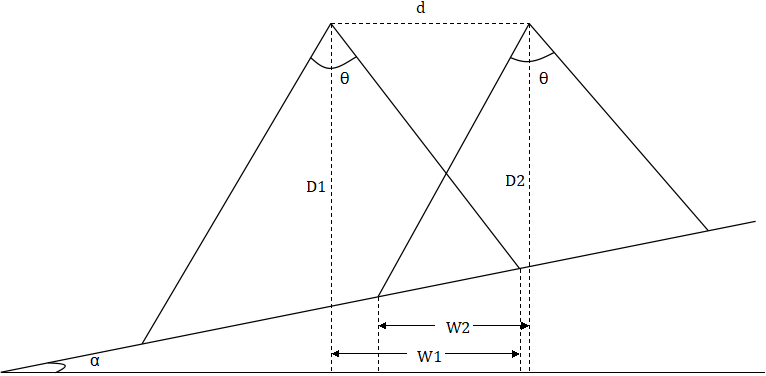
\includegraphics[width=9cm]{figures/几何分析示意图.png}
		\caption{几何分析示意图}\label{img001}
	\end{figure}

如图~\ref{img001}~所示，在海底存在一定坡度的基础上，当多波束测量船在不同位置时，其测量的海底深度存在差异，而不同位置的海水深度之间包含着几何关系。图中取了两处测量点，两处测线间距为$d$，坡度设为$\alpha$,两处测量点的海水深度分别记为$D_1$,$D_2$，则条带覆盖宽度可用图中符号表示为$W=W_1+W_2-d$。
对于$D_1,W_1$和$W_2,D_2$分别可以通过正弦定理列出含有参数$\theta$和$\alpha$的等式，记为式~\ref{equ001}~。

\begin{equation}\label{equ001}
	\begin{aligned}
		\frac{\sin (90^\circ+\alpha-\theta / 2)}{D_1}&=\frac{\sin (\theta / 2)}{W_1 / \cos \alpha}\\
		\frac{\sin (90^\circ-\alpha-\theta / 2)}{D_2}&=\frac{\sin (\theta / 2)}{W_2 / \cos \alpha}
	\end{aligned}
\end{equation}

将式子~\ref{equ001}变形得到式子~\ref{equ002}~。

\begin{equation}\label{equ002}
	\begin{aligned}
		W_1&=D_1*(\sin (\theta / 2) / \sin (90^\circ+\alpha-\theta / 2))* \cos \alpha\\
		W_2&=D_2*(\sin (\theta / 2) / \sin (90^\circ-\alpha-\theta / 2))* \cos \alpha
	\end{aligned}
\end{equation}

最终通过$W=W_1+W_2-d$,就能得到条带覆盖宽度与海水深度的数学关系。

\subsubsection{重叠率计算}

已知，当测线平行且海底地形平坦的情况下，相邻条带之间的重叠率由公式~\ref{equ003}~定义。
\begin{equation}\label{equ003}
	\eta=1-\frac{d}{W}
\end{equation}
其中$d$为相邻两条测线的间距，$W$为条带的覆盖宽度。但海底地形在真实环境中难免会存在起伏，地形平坦只是海底地形的一种特殊情况，在本题中海底地形有一定的坡度，故在计算$W$的过程中，我们引入了$W_1$和$W_2$,以确保重叠率的准确性，最终得到公式~\ref{equ004}~。
\begin{equation}\label{equ004}
	\eta=(W_1+W_2-d)/(W_1+W_2)
\end{equation}

联立公式~\ref{equ002}~和~\ref{equ004}~，我们最终得到了计算多波束测深覆盖宽度及重叠率的数学模型。
\subsubsection{模型求解}
已知多波束换能器的开角为$120^\circ$，坡度为$1.5^\circ$，海水深度在海域中心点处为$70m$，将题中给出的不同的测线距中心点处的距离带入数学模型中，所得结果如
表~\ref{tab002}~(结果保留三位小数)所示：
\begin{table}[!htbp]
	\centering
	\caption{result1}\label{tab002}
	 \resizebox{\textwidth}{!}{
	\begin{tabular}{|c|c|c|c|c|c|c|c|c|c|} 
		\toprule
		测线距中心点处的距离/m  & -800    & -600    & -400    & -200    & 0       & 200     & 400     & 600     & 800      \\ 
		\hline
		海水深度/m        & 90.948  & 85.712  & 80.474  & 75.237  & 70      & 64.763  & 59.526  & 54.288  & 49.051   \\ 
		\hline
		覆盖宽度/m        & 315.702 & 297.527 & 279.345 & 261.166 & 242.986 & 224.808 & 206.629 & 188.447 & 170.268  \\ 
		\hline
		与前一条测线的重叠率/\% & ——      & 34.683  & 30.561  & 25.883  & 20.529  & 14.341  & 7.109   & -1.458  & -11.766  \\
		\bottomrule
	\end{tabular}
}
\end{table}
\subsection{问题二的模型建立与求解}
\subsubsection{模型的建立}
\begin{figure}[h]
	\small
	\centering
	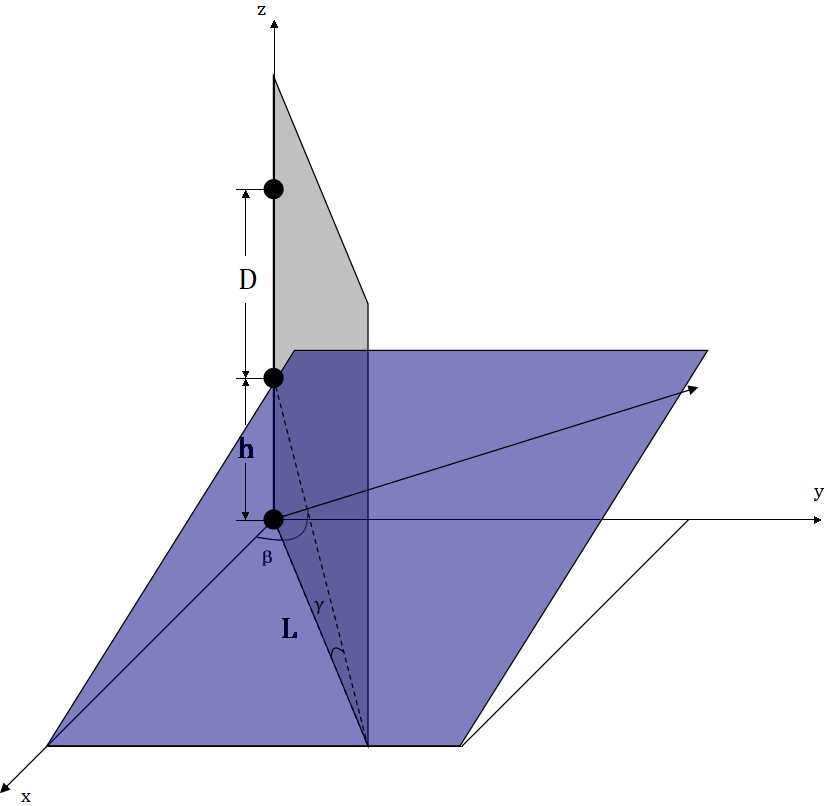
\includegraphics[width=9cm]{figures/立体分析示意图.png}
	\caption{立体分析示意图}\label{img002}
\end{figure}

由于在测量矩形海域时，测量方向可以选择为任意方向，每当方向发生改变时，与测线方向垂直的平面和坡面的夹角也会发生改变，即在不同测线方向上会存在不同
的坡度。由方程~\ref{equ002}~和~\ref{equ004}~可知，将已知坡度代入，便可得到覆盖宽度的大小。而测线方向与海底坡面的法向在水平面上投影的夹角为与测线方向具有一定的关
系，可通过夹角 判断测线方向，所以在本文中，我们需要建立夹角 与坡度之间的几何关系。

如图~\ref{img002}~所示，由矩形海域在水平面的投影可以得到三角关系式~\ref{equ005}~。
\begin{equation}\label{equ005}
	\begin{aligned}
		\frac{h/tan\alpha}{L}=cos(\beta-90^\circ)
	\end{aligned}
\end{equation}

进一步推算出式~\ref{equ006}~。
\begin{equation}\label{equ006}
	\begin{aligned}
		\frac{h}{L}=tan\alpha*sin\beta=tan\gamma
	\end{aligned}
\end{equation}

接下来我们从图中可以寻找到对于任意角度的$D_i$与$D_0$满足关系~\ref{equ007}~，其中$d_i$表示测线距中心点处的距离。
\begin{equation}\label{equ007}
	\begin{aligned}
		D_i=D_0-tan\gamma*d_i
	\end{aligned}
\end{equation}

同时，通过第一问我们推导出了$W_i$与$D_i$的关系，如式~\ref{equ008}~所示。
\begin{equation}\label{equ008}
	\begin{aligned}
		W_i=D_i*sin(\theta/2)*(\frac{1}{sin(90^\circ+\alpha-\theta/2)}+\frac{1}{sin(90^\circ-\alpha-\theta/2)})*cos\alpha
	\end{aligned}
\end{equation}

联立方程~\ref{equ006}~,~\ref{equ007}~,~\ref{equ008}~，便得到了解决矩形海域多波束测深覆盖宽度问题的数学模型。
\subsubsection{模型的求解}

\begin{table}[!htbp]
	\centering
	\caption{result2}\label{tab003}
	 \resizebox{\textwidth}{!}{
	\begin{tabular}{|c|c|c|c|c|c|c|c|c|c|} 
		\hline
		\multicolumn{2}{|c|}{\multirow{2}{*}{覆盖宽度/m}} & \multicolumn{8}{c|}{测量船距海域中心点处的距离/海里}                                          \\ 
		\cline{3-10}
		\multicolumn{2}{|c|}{}                        & 0       & 0.3     & 0.6     & 0.9     & 1.2     & 1.5     & 1.8     & 2.1      \\ 
		\hline
		\multirow{8}{*}{测线方向夹角/°} & 0                 & 415.692 & 415.692 & 415.692 & 415.692 & 415.692 & 415.692 & 415.692 & 415.692  \\ 
		\cline{2-10}
		& 45                & 416.120 & 380.446 & 344.772 & 309.098 & 273.424 & 237.750 & 202.076 & 166.402  \\ 
		\cline{2-10}
		& 90                & 416.549 & 366.046 & 315.544 & 265.041 & 214.538 & 164.035 & 113.533 & 63.030   \\ 
		\cline{2-10}
		& 135               & 416.120 & 380.446 & 344.772 & 309.098 & 273.424 & 237.750 & 202.076 & 166.402  \\ 
		\cline{2-10}
		& 180               & 415.692 & 415.692 & 415.692 & 415.692 & 415.692 & 415.692 & 415.692 & 415.692  \\ 
		\cline{2-10}
		& 225               & 416.120 & 451.794 & 487.468 & 523.142 & 558.816 & 594.491 & 630.165 & 665.839  \\ 
		\cline{2-10}
		& 270               & 416.549 & 467.052 & 517.555 & 568.057 & 618.560 & 669.063 & 719.566 & 770.068  \\ 
		\cline{2-10}
		& 315               & 416.120 & 451.794 & 487.468 & 523.142 & 558.816 & 594.491 & 630.165 & 665.839  \\
		\hline
	\end{tabular}
}
\end{table}

已知多波束换能器的开角为$120^\circ$，坡度为$1.5^\circ$，海水深度在海域中心点处为$120m$，即$\theta=120^\circ,\alpha=1.5^\circ,D=120m$,并且题表中已经给出了不同测线方向夹角$\beta$和测线距中心点处的距离$d_i$，我们将以上参数带入数学模型当中，所得结果如表~\ref{tab003}~所示。
\subsection{问题三的模型建立与求解}
\subsubsection{确定最优测线方向}
图~\ref*{img003}~是用于判断最优测线方向的示意图。
\begin{figure}[h]
	\small
	\centering
	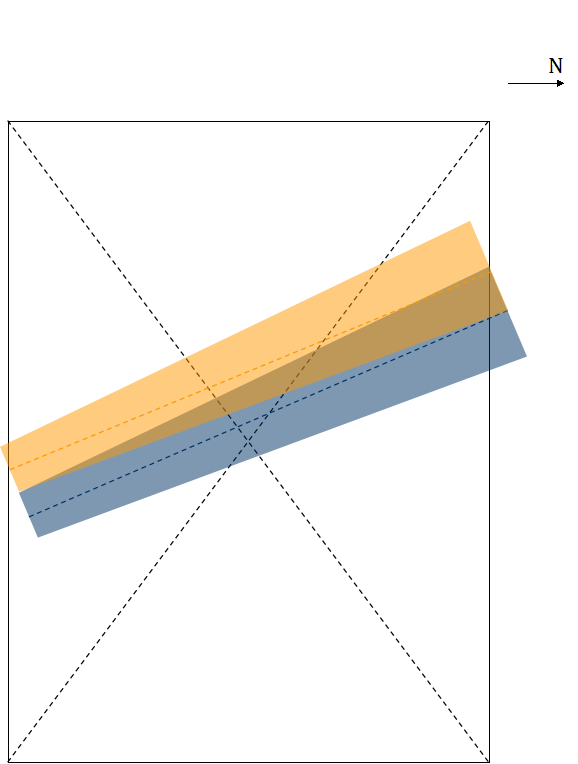
\includegraphics[width=9cm]{figures/测线方向分析示意图.png}
	\caption{测线方向分析示意图}\label{img003}
\end{figure}

在坡度的影响下，$\beta$为不同类型角度时，所确定最优测线方向可能存在差异，于是我们将此问题进行分类讨论，即当$\beta$为非直角时及当$\beta$为直角时两种情况。

(1)$\beta$为非直角时。

待测海域投影为图~\ref{img003}~中矩形底图，左右为南北朝向，该图中从下到上由浅至深（根据对称性，反之同理）。经过资料\cite{bib:one}查询得知，测线方向一定是一组平行线。如图中橙色部分与蓝色部分矩形上下底中点连线平行所示。橙色部分与蓝色部分就是以这两条平行线为轴线构成的具有一定宽度的全覆盖水深条带。其中阴影部分则是测量船测量重叠的区域，其构成了一个三角形。当三角形左侧的顶点位于矩形内部时，则将出现漏侧的情况。故阴影三角形左侧顶点应处于矩形边界甚至边界以外。但是，当左侧顶点处于边界以外时，当测量船测量结束，矩形左边界处，会存在重叠率。此时，相邻测线之间的距离会相比于阴影三角形左侧顶点恰处于矩形边界这一情况时小。而若想设计处一组测量长度最短的测线，相邻测线之间的距离应当越大越好。故无漏测无重叠率是测线之间的距离为最佳距离。

接下来调整测线方向，随着测线方向越接近南北方向时，即$\beta$越接近$90^\circ$,其测线的最佳距离会进一步减少。

(2)$\beta$为直角时。

由$\beta$为非直角时这一情况可以得到，$\beta$越接近$90^\circ$,其测线的最佳距离会进一步减少。综上，我们可得在界状态求下当$\beta$为直角时，即$\beta$=$90^\circ$时，测线方向为最优方向。

\subsubsection{模型求解}

已经得出结论，当$\beta$为直角时，拥有最优测线方案。即测线方向由南向北。在测量船由南向北行驶过程中，东西方向无非是由浅到深（如图所示）或由深到浅，根据对称性，二者结论应当是相同的。此处我们只研究前者状况。

首先根据公式~\ref{equ003}~：$\eta=1-\frac{d}{W}$,以及题中重叠率位于$10\%\sim20\%$条件可知，为了使相邻测线距离$d$越大，我们取重叠率为$10\%$，得到$d=0.9W$。此时满足公式~\ref{equ002},且有：

\begin{equation}\label{equ009}
	W=(W_1+W_2)cos\alpha
\end{equation}

同时，联立公式~\ref{equ007}~进行求解。

通过python迭代求解，最终得到n=32，最短测量路径总长度为$118528m$。

\begin{figure}[h]
	\small
	\centering
	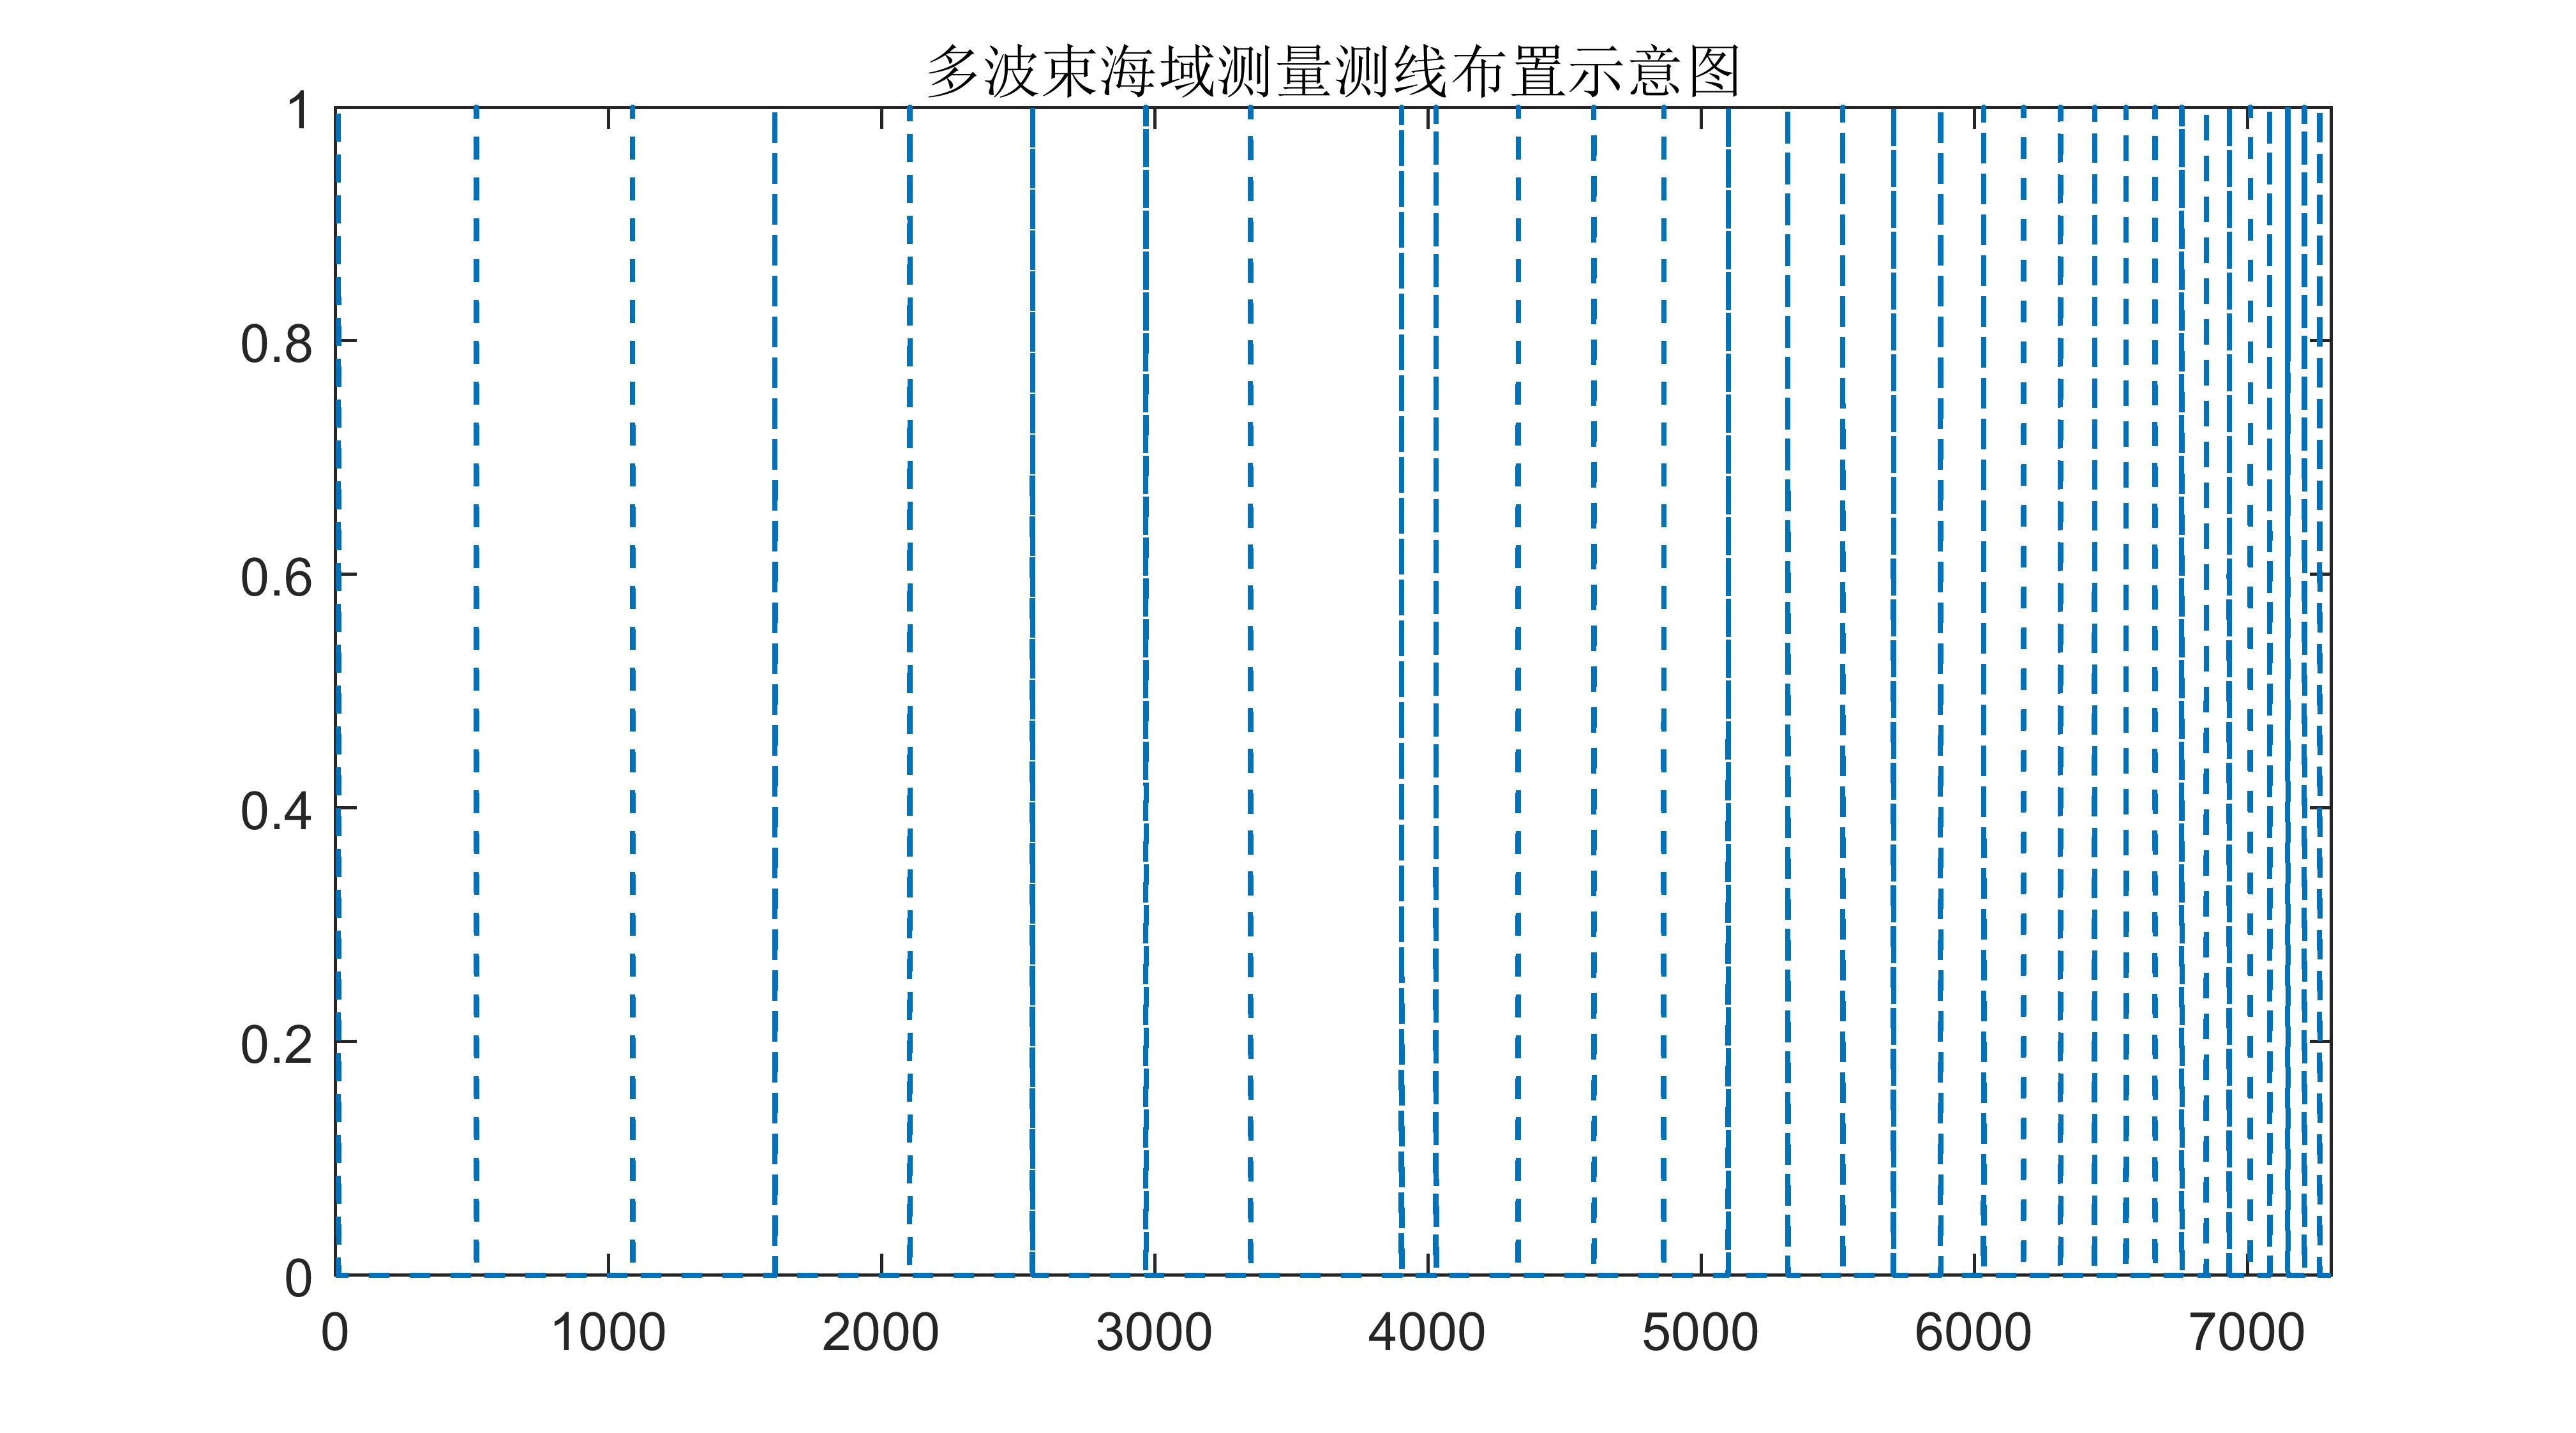
\includegraphics[width=11cm]{figures/结果图.jpg}
	\caption{测线分布示意图}\label{img004}
\end{figure}

至此，即得到测量长度最短，可完全覆盖整个待测海域，且相邻条带之间的重叠率满足$10\%\sim20\%$的测线，如图~\ref{img004}~所示。

\subsection{问题四的建立与求解}
\subsubsection{数据预处理与模型建立}

为了题目所提供数据展示更加直观，我们先利用由单波束测量的测深数据对海深进行取负数操作。利用 MATLAB 绘制该待测海域的海底三维图和等深线图。如下图所示：
\begin{figure}[htbp]
	\centering
	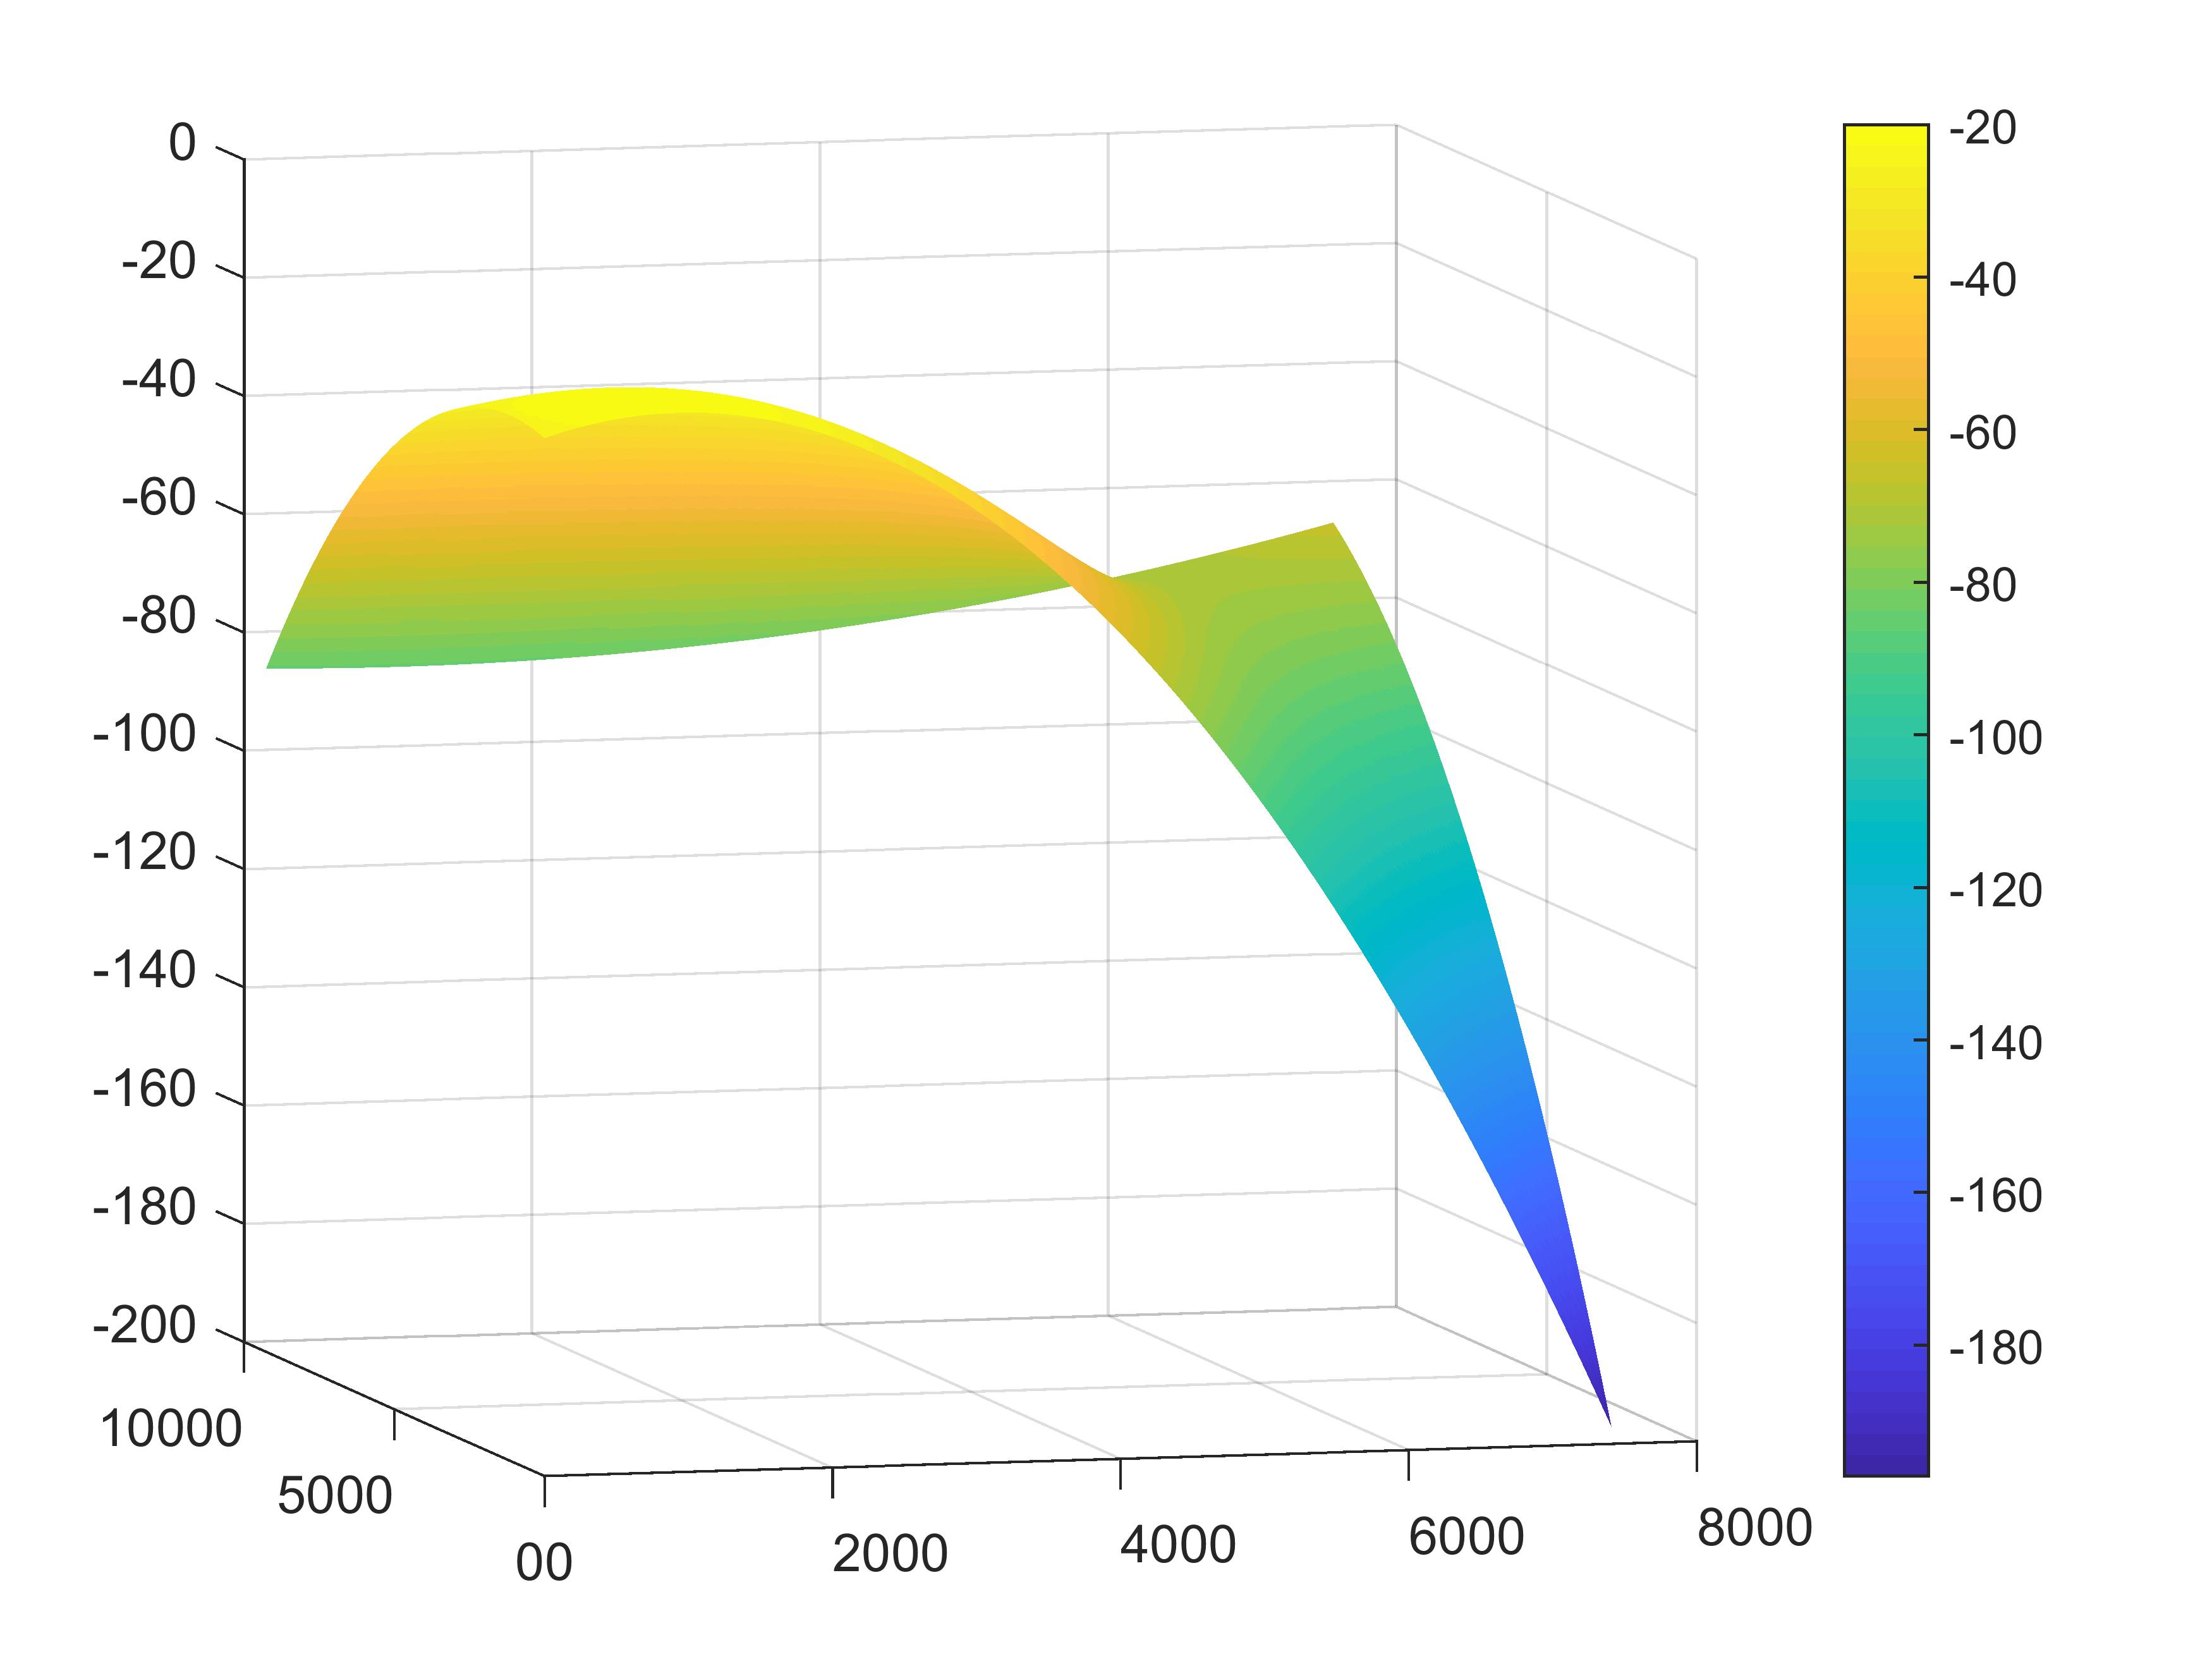
\includegraphics[width=7cm]{figures/视图1.jpg}
	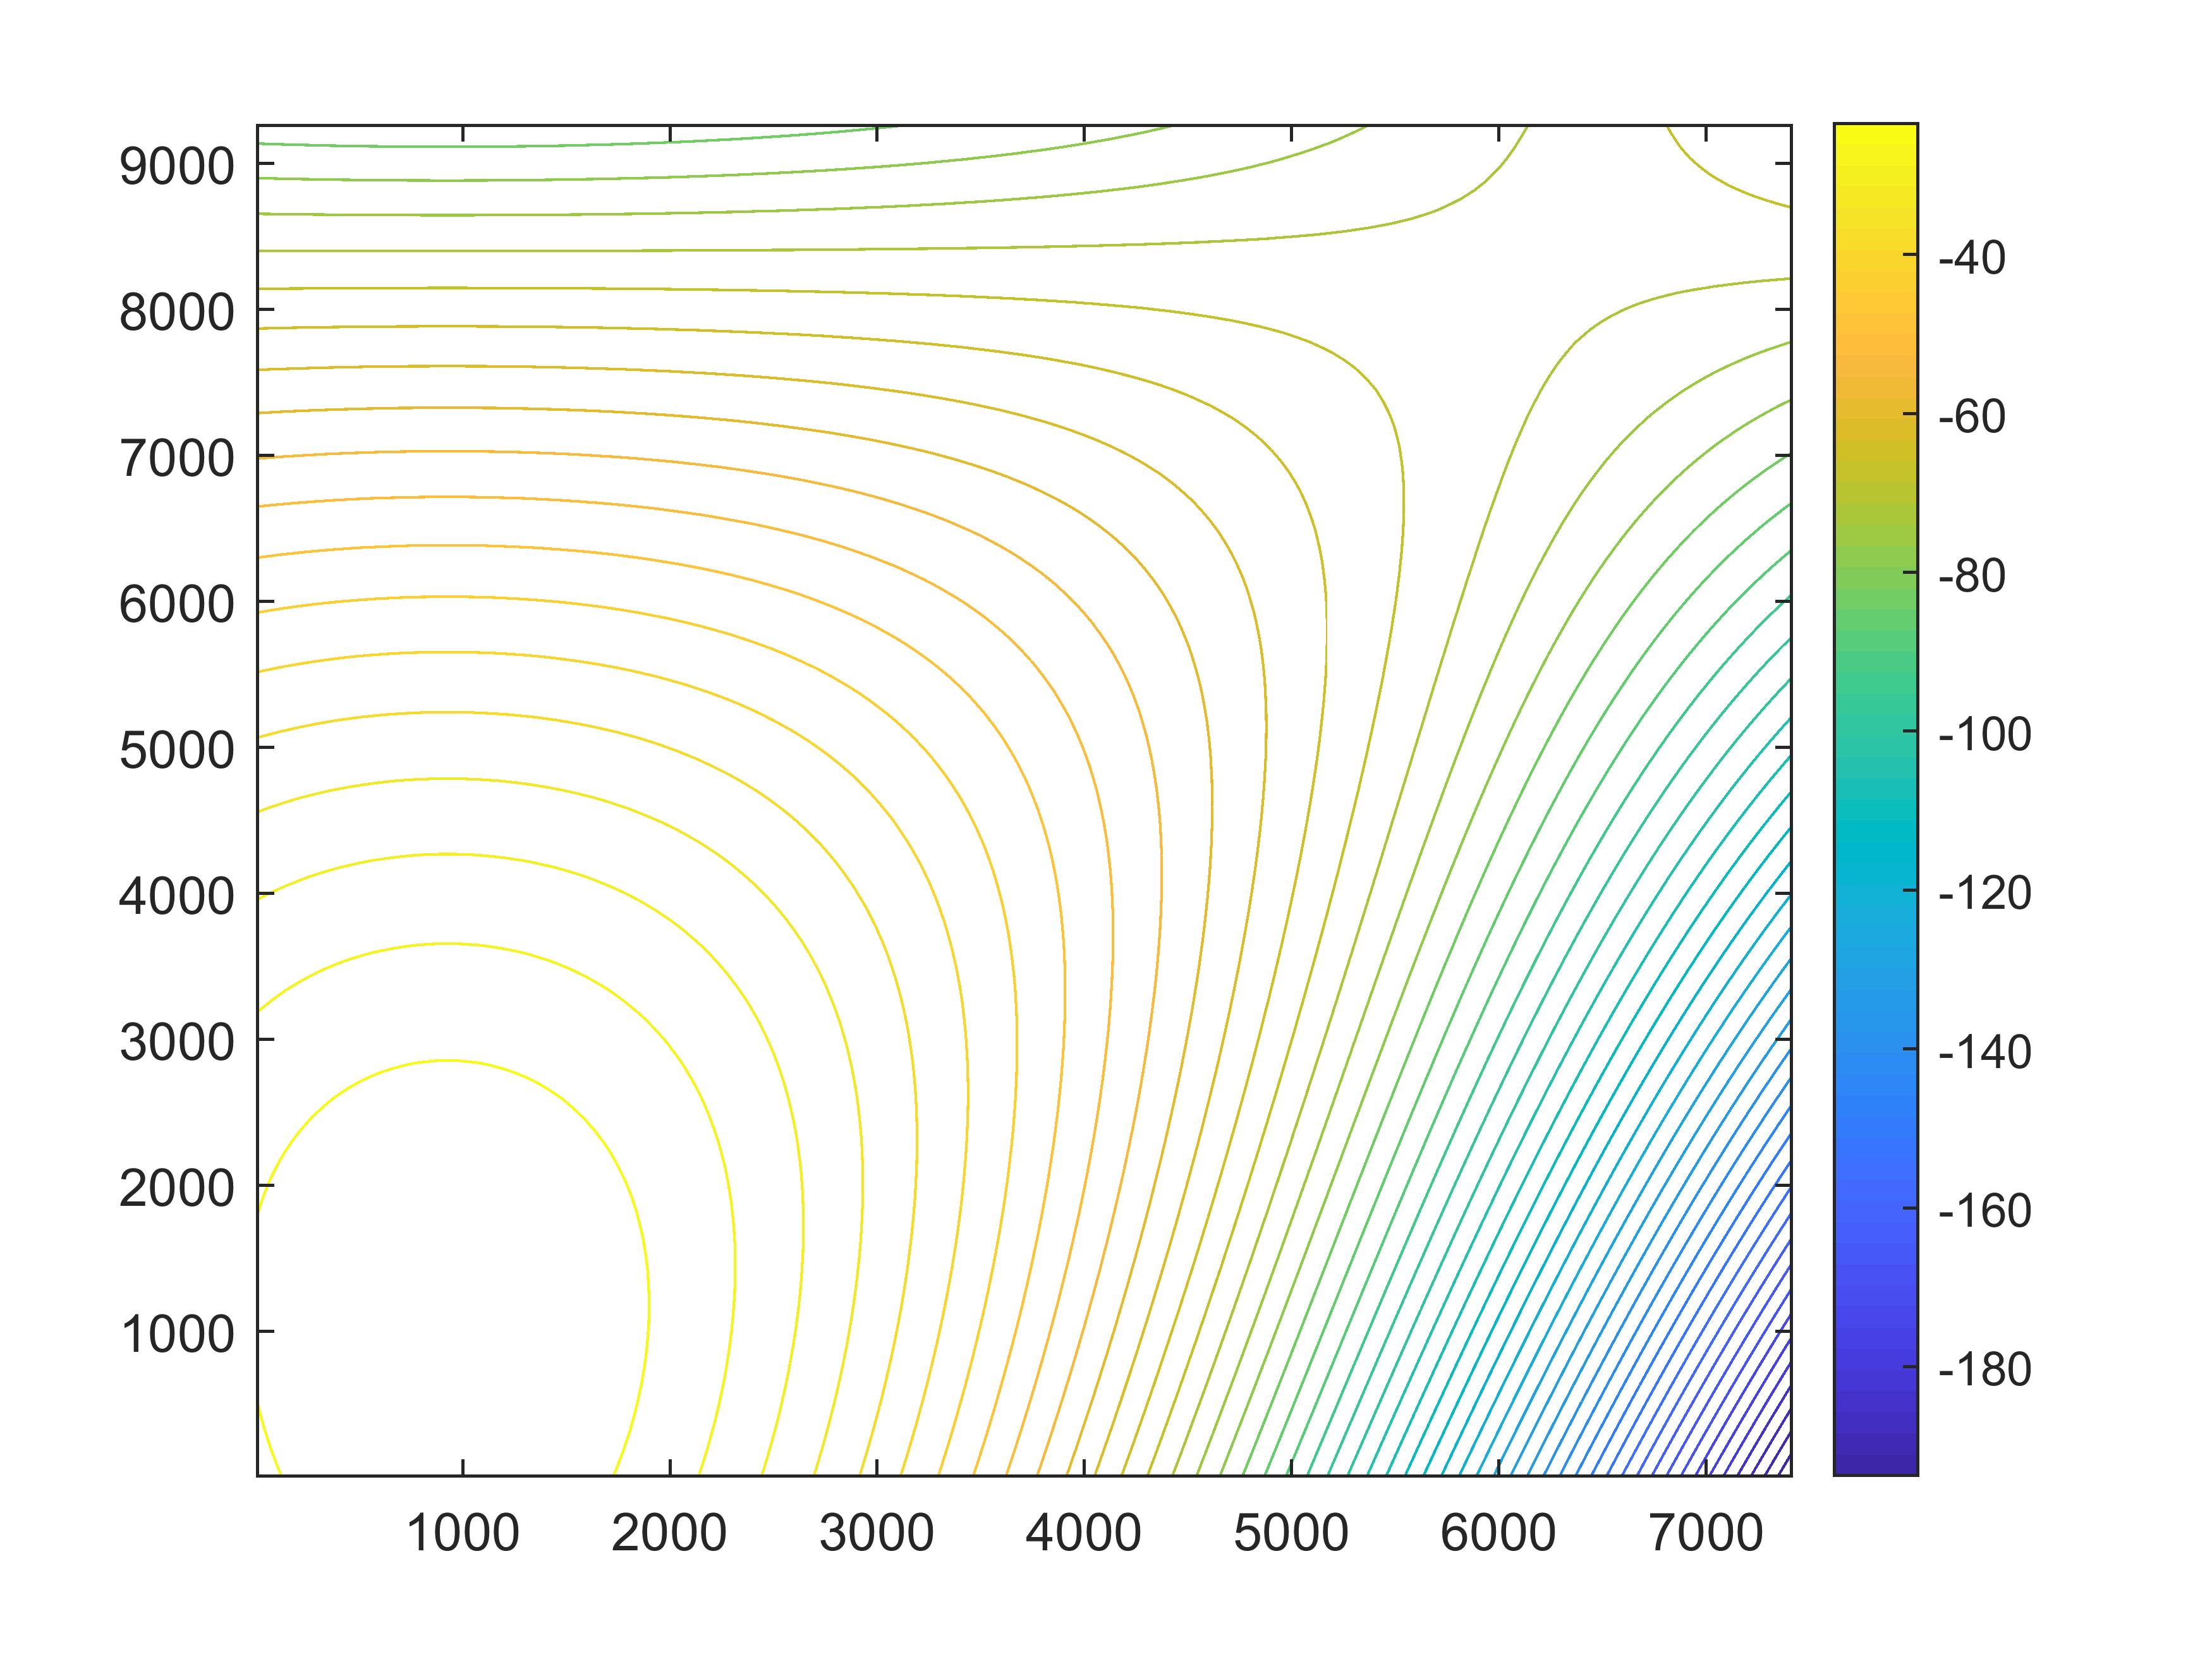
\includegraphics[width=7cm]{figures/视图2.jpg}
	\caption{相对高度示意图}
\end{figure}

左侧图是一个三维海底面分布视图，很明显，海底海底的地形起伏较大，呈现不规则分布。右侧图是一个海底地形的等深线分布视图。

针对问题四中描述的复杂海域地形，其特征在于显著的水深起伏变化。在规划测线布局时，若单纯依赖海域的平均水深作为布设基准，将面临双重挑战：在浅水区域，易导致探测盲区，影响数据完整性，从而降低探测质量；而在深水区域，则可能因测线过密而造成相邻探测条带间不必要的重叠，这一现象不仅浪费资源，还显著降低了探测效率。

\begin{figure}[htbp]
	\centering
	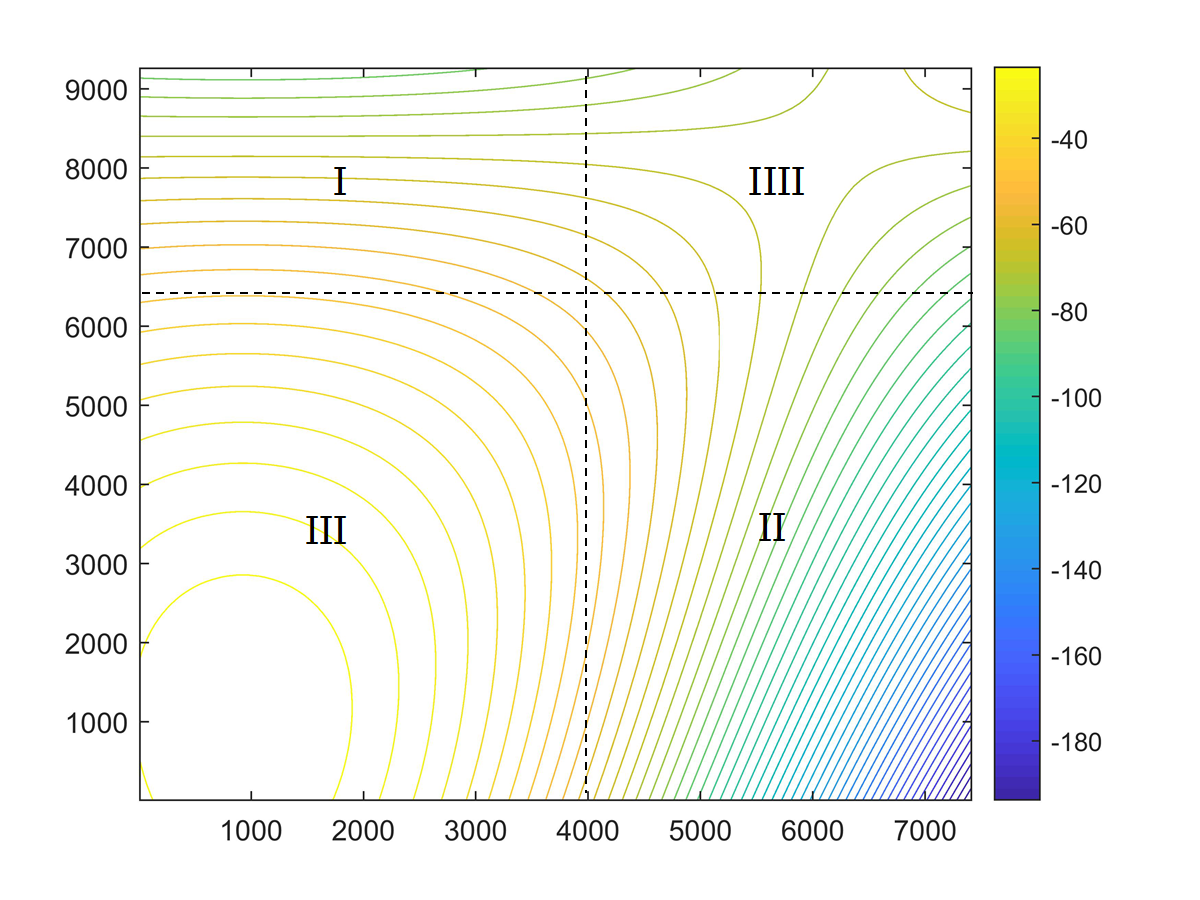
\includegraphics[width=9cm]{figures/图片1.png}
	\caption{海域划分图示}\label{img005}
\end{figure}

为了全面覆盖目标海域并优化探测效率，科学设定测线间隔成为关键。受问题三模型提供的启示，我们采取了一种策略性的海域划分方法，即将整体海域人为地划分为四个矩形子区域,如图~\ref{img005}~所示。这一划分的核心原则在于确保矩形的一边尽可能与等深线走向保持一致，以此最大化地适应并反映海域的实际地形特征。如图右侧所示，通过这种精细划分，我们得以对每个子区域实施更为针对性的测线布设策略。

接下来，针对每个子区域，我们将分别进行细致的测线规划，旨在最小化漏测区域的同时，将相邻条带的重叠率控制在合理范围内（如不超过20\%），以此平衡探测的完整性与效率。

对于图中四个区域，我们打算将其分别拟合成坡面以利用前文模型求解。在三维坐标系中， 设海底矩形平面的方程为 z = Ax + By + C ，采用最小二乘法，通过附件所给的海水深度数据，对坡面方程的参数 A 、B 、C 进行估计。

对于每一部分的矩形坡面都可以利用第三问的数学模型，以测线的总长度最小为优化目标，将相邻条带之间的重叠率尽量控制在20\%以下和沿测线形成的条带尽可能覆盖整个待测海域为约束条件，建立单目标优化模型进行求解。

\subsubsection{模型求解}

由于区域4的拟合效果极差，故采用区域1测线的延长线作为区域4的测线。最终得到结果如~\ref{tab004}~所示。
\begin{table}[!htbp]
	\centering
	\caption{第四问模型求解结果示意}\label{tab004}
	\resizebox{\textwidth}{!}{
		\begin{tabular}{|c|c|c|c|c|c|} 
			\toprule
			 \quad  & 测线数量    & 漏测面积/$m^2$    & 漏测面积占总面积的百分比/\%    & 重叠率超过20\%的长度/m    & 夹角/°         \\ 
			\hline
			区域1、4        & 53  & 3068210  & 0.22703  & 70128  & 0.11424763      \\ 
			\hline
			区域2        & 68 & 0 & 0 & 0 & 0.1745224  \\ 
			\hline
			区域3 & 168      & 0  & 0  & 0  & 1.15378102    \\
			\bottomrule
		\end{tabular}
	}
\end{table}

由上表可得，该海域的测线的总长度为356079m、漏测海区面积为$3068210m^2$，占总面积百分比为$22.7\%$以及重叠率超过20\%部分的总长度为70128m。

\subsubsection{结果分析}
区域3的测线极多。这是因为区域3与水平面的夹角很大，即区域3很陡，使得多波束打到区域3底面的波束宽度很小。又因为区域3的范围较大，这就需要布设许多测线才能使得沿测线扫描形成的条带尽可能地覆盖整个区域3。

区域1，4出现大量漏测，这是因为该区域的海底地形较为复杂，等深线方向极为不一致，为了降低测量工作难度，我们采用区域 I 的测线延伸线作为该区域的测线。区域 I 相比，该区域海水较浅，故出现漏测的情况。

区域2，3并没有出现漏测区域。这是因为对于划分的矩形区域，我们是基于贪心算法循环遍历求解测线间距的，该算法会始终让沿测线扫描形成的条带覆盖整个矩形区域。


\section{结果分析与模型评价}
\subsection{模型检验及可靠性分析}
\subsubsection{模型检验}

\textbf{数据验证}：首先，对多波束测深覆盖宽度及重叠率模型进行了理论验证。通过对比模型计算结果与已知理论值（如几何三角函数关系等），确认模型在理论层面上的正确性。结果显示，模型计算出的覆盖宽度和重叠率与理论预期高度一致，验证了模型的理论基础。

\textbf{敏感性分析}：对模型中的关键参数（如换能器开角、海底坡度、海域中心点水深等）进行了敏感性分析。通过调整这些参数的值，观察模型输出结果的变化情况。结果显示，模型对参数的变化具有较高的敏感性，且变化趋势符合物理规律，进一步验证了模型的可靠性。

\subsubsection{可靠性分析}

\textbf{数据可靠性}：模型所依赖的数据来源可靠，包括实际测量的多波束测深数据和海底地形图等。这些数据均经过严格的质量控制和验证，确保了数据的准确性和可靠性。同时，在数据处理过程中采用了先进的算法和技术手段，进一步提高了数据的可靠性。

\textbf{模型稳定性}：对模型进行了多次重复运行和测试，观察模型输出结果的稳定性。结果显示，在不同运行条件下，模型输出结果均保持一致性和稳定性，未出现明显的波动或异常现象。这表明模型具有较高的稳定性和可靠性。

\subsection{模型评价与推广}
\subsubsection{模型优点}
\textbf{准确性}：本模型基于多波束测深技术的核心参数（如换能器开角、海底坡度、海水深度等），全面考虑了影响覆盖宽度和重叠率的各种因素，能够较为准确地计算出在不同条件下的覆盖宽度和重叠率，为测线规划提供了可靠的理论依据。

\textbf{灵活性}：模型不仅适用于平坦海底的测线规划，还通过引入坡度因素，能够灵活应对复杂多变的海底地形，确保测量数据的全面覆盖和准确性。

\textbf{高效性}：通过数学建模和算法优化，本模型能够在较短时间内完成大量计算，为实际测量工作提供了高效的测线布局方案，提高了测量效率。


\subsubsection{缺陷}

\textbf{假设条件限制}：模型在建立过程中做了一定的假设和简化，如假设海底坡度在一定范围内均匀变化，未充分考虑海底地形的极端复杂性和不确定性，这可能导致在某些极端情况下模型的预测精度降低。

\textbf{数据依赖性}：模型的准确性和可靠性高度依赖于输入数据的准确性和完整性。如果输入数据存在误差或缺失，将直接影响模型的预测结果和测线布局的合理性。

\textbf{计算复杂度}：随着海域面积和测量要求的增加，模型的计算量也会显著增加，可能导致计算时间延长和资源消耗增加。

\subsubsection{模型改进}

\textbf{引入更精细的地形数据}：模通过获取更高分辨率的海底地形数据（如多波束测深数据、侧扫声呐数据等），并结合地理信息系统（GIS）技术，对海底地形进行更精细的建模和分析，以提高模型的预测精度和适应性。

\textbf{考虑更多影响因素}：在模型建立过程中，可以进一步考虑其他可能影响覆盖宽度和重叠率的因素，如水流速度、海底沉积物类型等，以提高模型的全面性和准确性。此外，还可以引入机器学习和人工智能技术，对模型进行智能优化和自适应调整。

\begin{thebibliography}{9}%宽度9
	\bibitem{bib:one} JT/T 790-2010, 多波束测深系统测量技术要求[S].
\end{thebibliography}
\newpage
%附录
\begin{appendices}
	\section{第一题}
	\subsection{代码}
	\begin{lstlisting}[language=python]
		import math
		D=90.948
		degree=120
		alpha=1.5
		d=200 #船距海域中心点处的距离
		
		#B题第一问
		def Cal_W(alpha,D,degree): #计算覆盖宽度
		W=math.cos(math.radians(alpha))*D*math.sin(math.radians(degree/2))*(1/math.sin
		(math.radians(90-alpha-degree/2))+1/math.sin(math.radians(90+alpha-degree/2)))
		return W
		
		def Upper_W(alpha,D,degree):
		W=math.cos(math.radians(alpha))*D*math.sin(math.radians(degree/2))*1/math.sin
		(math.radians(90+alpha-degree/2))
		return W
		
		def Lowwer_W(alpha,D,degree):
		W=math.cos(math.radians(alpha))*D*math.sin(math.radians(degree/2))*1/math.sin
		(math.radians(90-alpha-degree/2))
		return W
		
		def Cal_n(alpha,D1,D2,degree,d): #计算重叠率(由下向上) D1>D2
		W1=math.cos(math.radians(alpha))*D1*math.sin(math.radians(degree/2))*1/math.sin
		(math.radians(90+alpha-degree/2))
		W2=math.cos(math.radians(alpha))*D2*math.sin(math.radians(degree/2))*1/math.sin
		(math.radians(90-alpha-degree/2))
		n=(W1+W2-d)/(W1+W2)
		return n
		
		print(Cal_n(1.5,90.948,85.712,120,200))
	\end{lstlisting}
	\subsection{结果}
	\begin{table}[!htbp]
		\centering
		\caption{result1}
		\resizebox{\textwidth}{!}{
			\begin{tabular}{|c|c|c|c|c|c|c|c|c|c|} 
				\toprule
				测线距中心点处的距离/m  & -800    & -600    & -400    & -200    & 0       & 200     & 400     & 600     & 800      \\ 
				\hline
				海水深度/m        & 90.948  & 85.712  & 80.474  & 75.237  & 70      & 64.763  & 59.526  & 54.288  & 49.051   \\ 
				\hline
				覆盖宽度/m        & 315.702 & 297.527 & 279.345 & 261.166 & 242.986 & 224.808 & 206.629 & 188.447 & 170.268  \\ 
				\hline
				与前一条测线的重叠率/\% & ——      & 34.683  & 30.561  & 25.883  & 20.529  & 14.341  & 7.109   & -1.458  & -11.766  \\
				\bottomrule
			\end{tabular}
		}
	\end{table}
	\section{第二题}
	\subsection{代码}
	\begin{lstlisting}[language=python]
		print(math.atan(math.sqrt(1))/math.pi*180)
		
		beta=[0,45,90,135,180,225,270,315]
		distance=[0,0.3,0.6,0.9,1.2,1.5,1.8,2.1]#船距海域中心点处的距离
		for i in range (len(beta)):
		for j in range(len(distance)):
		tan_gamma = math.tan(math.radians(alpha)) * math.sin(math.radians(beta[i]))
		gamma = math.atan(tan_gamma) / math.pi * 180
		D=120-tan_gamma*distance[j]*1852 #海里和米的单位转化
		print(Cal_W(gamma,D,degree))
		
		print(tan_gamma)
		print(gamma)
	\end{lstlisting}
	\subsection{结果}
	\begin{table}[!htbp]
		\centering
		\caption{result2}
		\resizebox{\textwidth}{!}{
			\begin{tabular}{|c|c|c|c|c|c|c|c|c|c|} 
				\hline
				\multicolumn{2}{|c|}{\multirow{2}{*}{覆盖宽度/m}} & \multicolumn{8}{c|}{测量船距海域中心点处的距离/海里}                                          \\ 
				\cline{3-10}
				\multicolumn{2}{|c|}{}                        & 0       & 0.3     & 0.6     & 0.9     & 1.2     & 1.5     & 1.8     & 2.1      \\ 
				\hline
				\multirow{8}{*}{测线方向夹角/°} & 0                 & 415.692 & 415.692 & 415.692 & 415.692 & 415.692 & 415.692 & 415.692 & 415.692  \\ 
				\cline{2-10}
				& 45                & 416.120 & 380.446 & 344.772 & 309.098 & 273.424 & 237.750 & 202.076 & 166.402  \\ 
				\cline{2-10}
				& 90                & 416.549 & 366.046 & 315.544 & 265.041 & 214.538 & 164.035 & 113.533 & 63.030   \\ 
				\cline{2-10}
				& 135               & 416.120 & 380.446 & 344.772 & 309.098 & 273.424 & 237.750 & 202.076 & 166.402  \\ 
				\cline{2-10}
				& 180               & 415.692 & 415.692 & 415.692 & 415.692 & 415.692 & 415.692 & 415.692 & 415.692  \\ 
				\cline{2-10}
				& 225               & 416.120 & 451.794 & 487.468 & 523.142 & 558.816 & 594.491 & 630.165 & 665.839  \\ 
				\cline{2-10}
				& 270               & 416.549 & 467.052 & 517.555 & 568.057 & 618.560 & 669.063 & 719.566 & 770.068  \\ 
				\cline{2-10}
				& 315               & 416.120 & 451.794 & 487.468 & 523.142 & 558.816 & 594.491 & 630.165 & 665.839  \\
				\hline
			\end{tabular}
		}
	\end{table}
	
	\section{第三题}
	\subsection{代码}
	\begin{lstlisting}[language=python]
		width=2*1852
		length=4*1852
		D=110
		cel_edge0=length/2+math.cos(math.radians(alpha))*D*math.sin(math.radians(degree/2))*1/
		math.sin(math.radians(90+alpha-degree/2)) #覆盖范围的上边沿，由海域中心开始
		flo_edge0=length/2-math.cos(math.radians(alpha))*D*math.sin(math.radians(degree/2))*1/
		math.sin(math.radians(90-alpha-degree/2))  #覆盖范围的下边沿，由海域中心开始
		print(cel_edge0)
		print(flo_edge0)
		cel_edge=cel_edge0
		print(cel_edge)
		flo_edge=flo_edge0
		
		d0=1
		while cel_edge<length: #先向上寻找
		D_temp=D-math.tan(math.radians(alpha))*1*d0  #以1m步长寻找10%重叠率的间隔位置
		d0+=1
		if (abs(Cal_n(alpha,D,D_temp,degree,d0))-0.1<0.012 and Cal_n(alpha,D,D_temp,degree,d0) >0.1) :
		#print(Cal_n(alpha,D,D_temp,degree,d0))
		# print("this is n")
		# print(Cal_n(alpha,D,D_temp,degree,d0))
		D=D_temp
		#print("this is D")
		#print(D)
		#print("this is d0")
		#print(d0)
		cel_edge+=d0
		print(cel_edge-cel_edge0+length/2)
		d0=1
		#print("------------")
		#print("end!")
		
		d0=1
		while flo_edge>0: #再向下寻找
		D_temp=D+math.tan(math.radians(alpha))*1*d0  #以1m步长寻找10%重叠率的间隔位置
		d0+=1
		if (abs(Cal_n(alpha,D_temp,D,degree,d0))-0.1<0.012 and Cal_n(alpha,D_temp,D,degree,d0) >0.1) :
		#print(Cal_n(alpha,D,D_temp,degree,d0))
		# print("this is n")
		# print(Cal_n(alpha,D,D_temp,degree,d0))
		D=D_temp
		#print("this is D")
		#print(D)
		#print("this is d0")
		#print(d0)
		flo_edge-=d0
		print(flo_edge-flo_edge0+length/2)
		d0=1
		#print("------------")
		print("end!")
	\end{lstlisting}
	\subsection{结果}
	\begin{figure}[h]
		\small
		\centering
		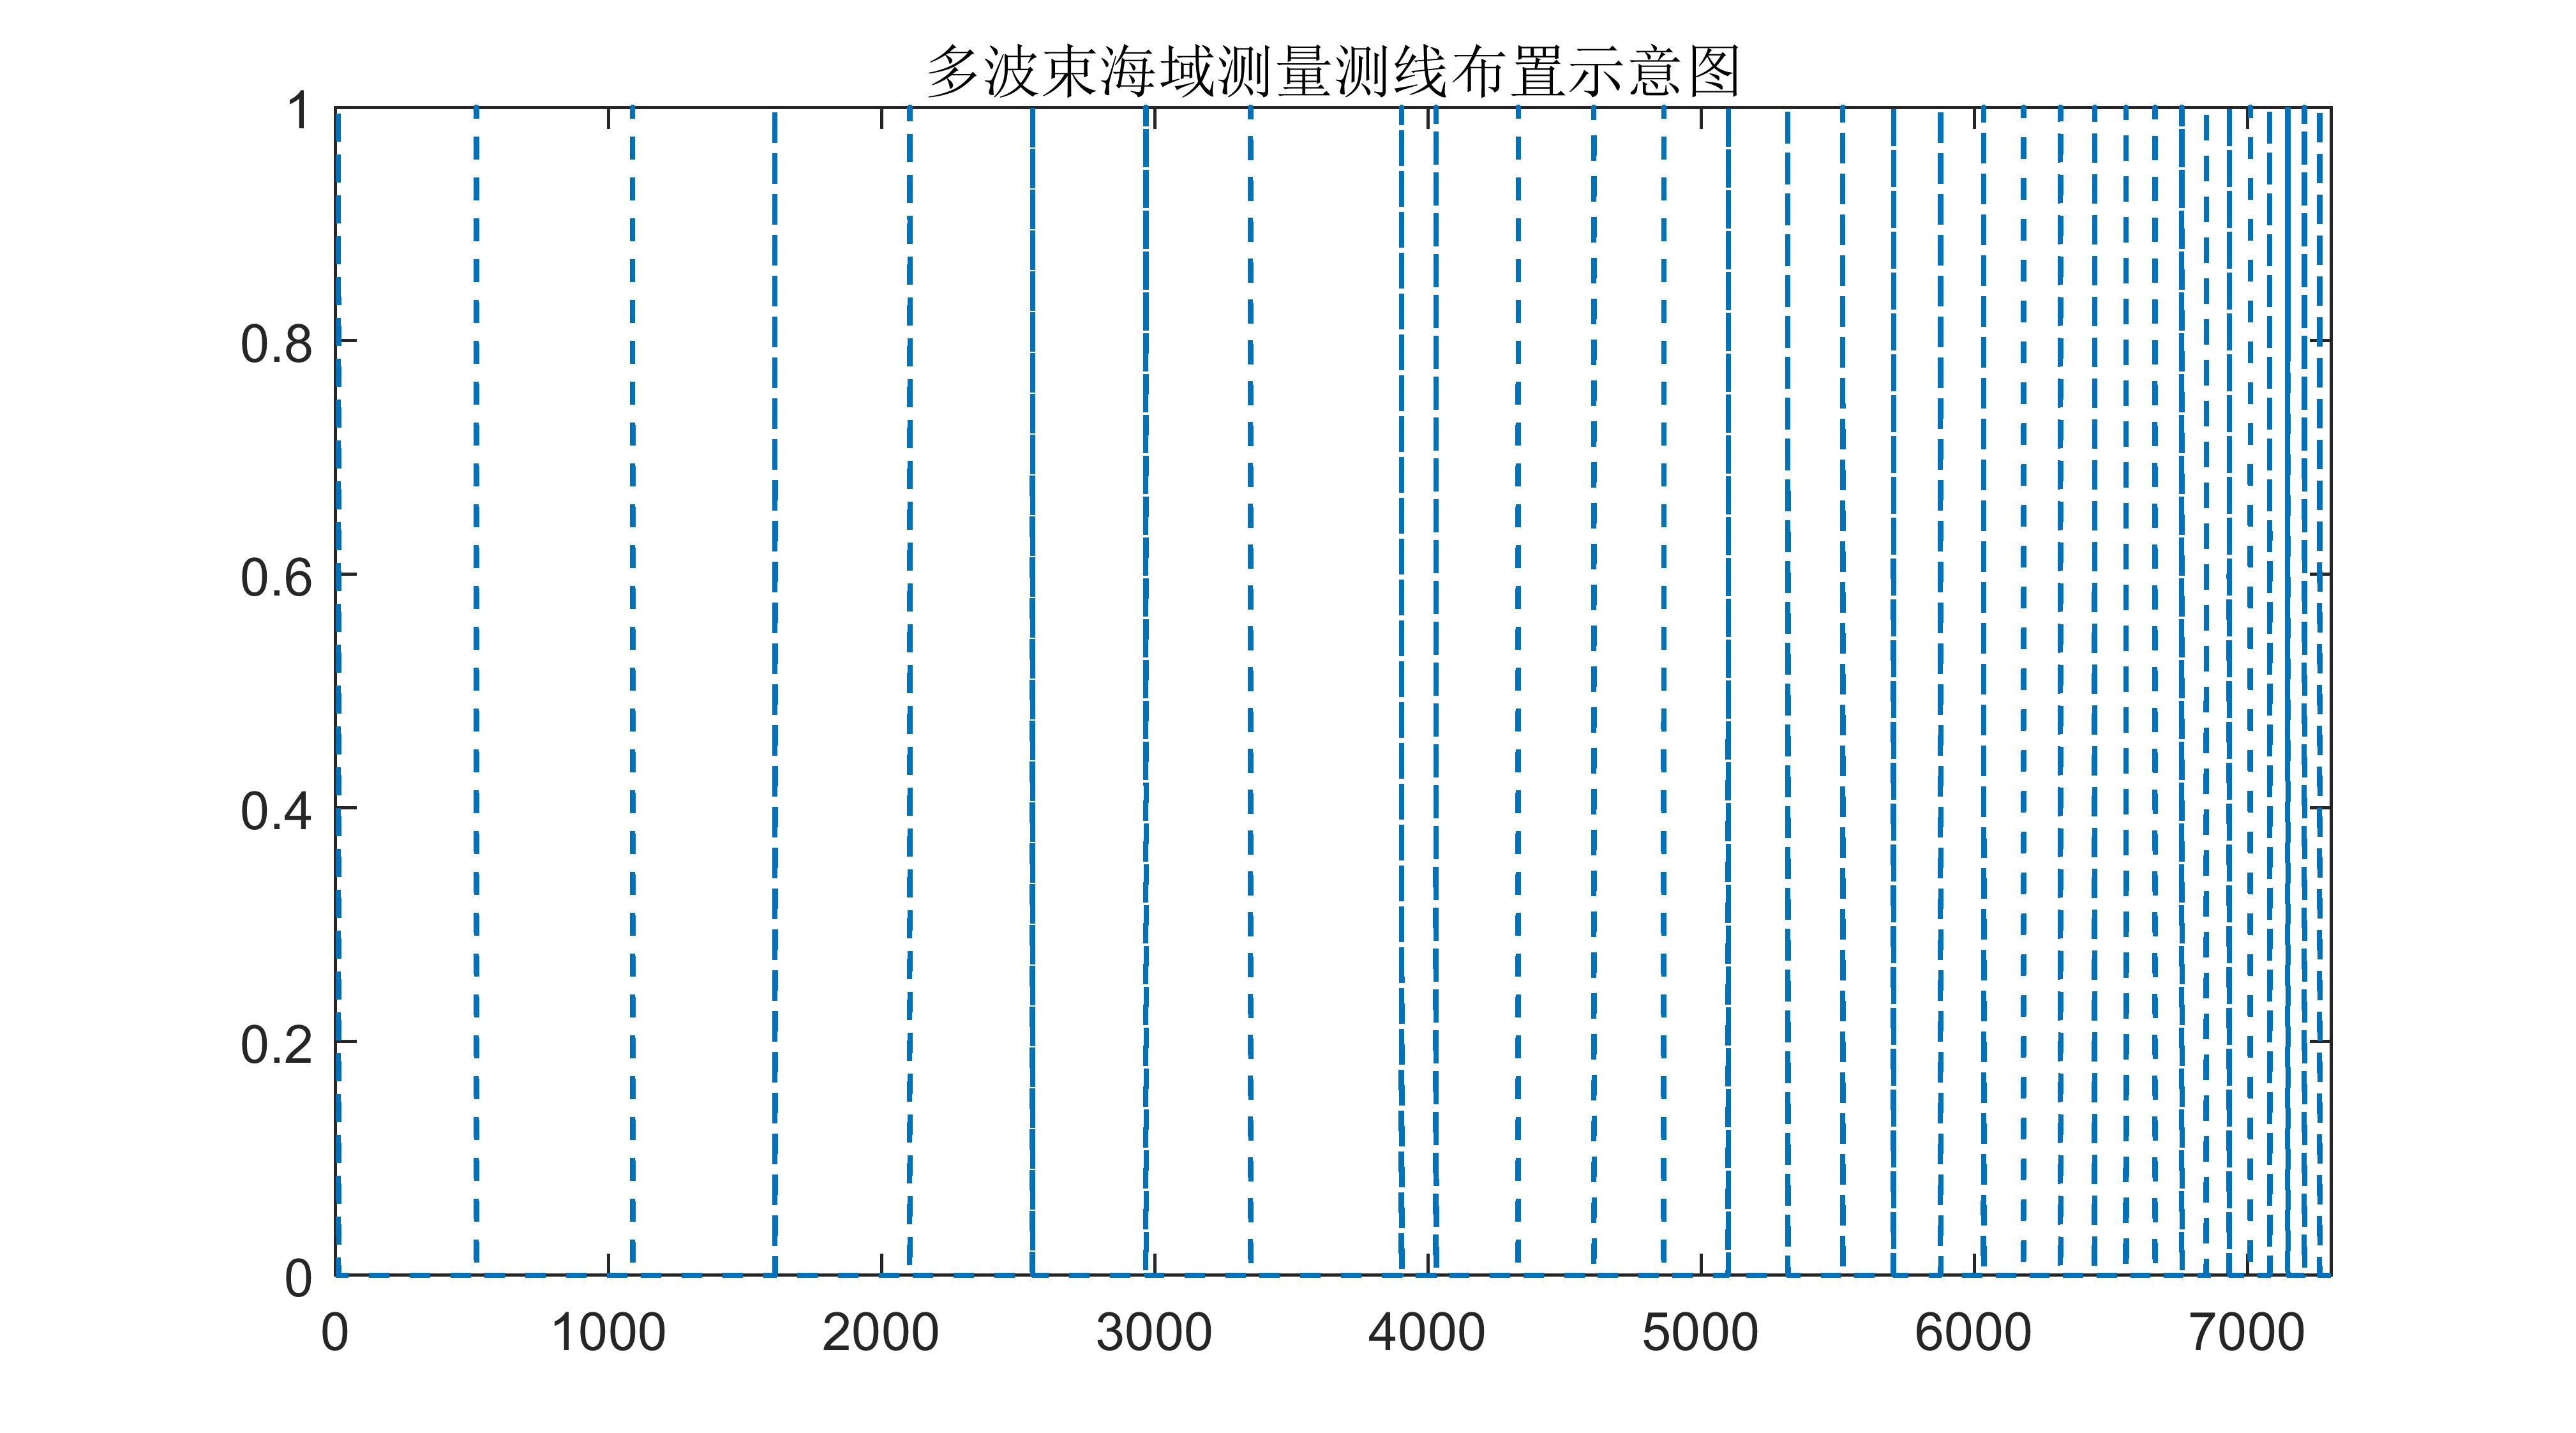
\includegraphics[width=13cm]{figures/结果图.jpg}
		\caption{测线分布示意图}
	\end{figure}
	\section{第四题}
	\subsection{代码}
	\begin{lstlisting}[language=python]
		#第四问漏测面积计算
		for i in range(length):
		for j in range(width):
		a_list = [1.3, 1.4, 1.5]
		for i in range(len(a_list)):
		a = a_list[i]
		b = 120
		radian1 = a * math.pi / 180
		radian2 = b / 2 * math.pi / 180
		D0 = 110
		Les = 4 * 1852  # 待测海域东西宽度
		D = D0 + Les / 2 * math.tan(radian1)  # 此处Dmax
		x = D * math.tan(radian2)
		D = D - x * math.tan(radian1)
		W1 = 0
		W2 = 0
		res_list = [x]
		left_list = []
		right_list = []
		
		while x + W2 * math.cos(radian1) <= Les:
		W2 = D * math.sin(radian2) / math.cos(radian2 - radian1)
		W1 = D * math.sin(radian2) / math.cos(radian2 + radian1)
		d = (W1 + W2) * 0.9 * math.cos(radian1) / (
		1 + math.sin(radian1) * math.sin(radian2) / math.cos(radian2 + radian1) * 0.9)
		left_list.append(x - W1 * math.cos(radian1))
		right_list.append(x + W2 * math.cos(radian1))
		D = D - d * math.tan(radian1)
		x = x + d
		res_list.append(x)
		
		W2 = D * math.sin(radian2) / math.cos(radian2 - radian1)
		W1 = D * math.sin(radian2) / math.cos(radian2 + radian1)
		d = (W1 + W2) * 0.9 * math.cos(radian1) / (
		1 + math.sin(radian1) * math.sin(radian2) / math.cos(radian2 + radian1) * 0.9)
		plt.plot(range(len(res_list)), res_list, linestyle='-', label=f'坡角为{a}°')
		
		plt.rcParams['font.sans-serif'] = ['SimHei']  # 指定默认字体
		plt.rcParams['axes.unicode_minus']
	\end{lstlisting}
	\subsection{结果}
	\begin{table}[!htbp]
		\centering
		\caption{第四问模型求解结果示意}\label{tab004}
		\resizebox{\textwidth}{!}{
			\begin{tabular}{|c|c|c|c|c|c|} 
				\toprule
				\quad  & 测线数量    & 漏测面积/$m^2$    & 漏测面积占总面积的百分比/\%    & 重叠率超过20\%的长度/m    & 夹角/°         \\ 
				\hline
				区域1、4        & 53  & 3068210  & 0.22703  & 70128  & 0.11424763      \\ 
				\hline
				区域2        & 68 & 0 & 0 & 0 & 0.1745224  \\ 
				\hline
				区域3 & 168      & 0  & 0  & 0  & 1.15378102    \\
				\bottomrule
			\end{tabular}
		}
	\end{table}
\end{appendices}
\end{document} 